\documentclass[
	11pt
	   t,
	aspectratio=169
]{beamer}

\graphicspath{{img/}}

\usepackage[alf]{abntex2cite}
\usepackage{booktabs} 
\usepackage{palatino} 
\usepackage[default]{opensans}
\usepackage{subcaption}
\usepackage[utf8]{inputenc}
\usepackage[russian]{babel}
\usepackage{tabto}
\usepackage{pgfplots}
\pgfplotsset{width=8cm,compat=1.9}
\usepgfplotslibrary{external}
\tikzexternalize
\usepackage[utf8]{inputenc}
\usepackage{listings}
\usepackage{xcolor}

\definecolor{vscBackground}{RGB}{255,255,255}    
\definecolor{vscKeyword}{RGB}{175,0,219}         
\definecolor{vscString}{RGB}{163,21,21}          
\definecolor{vscComment}{RGB}{0,128,0}           
\definecolor{vscFunction}{RGB}{121,94,38}        
\definecolor{vscNumber}{RGB}{9,134,88}           
\definecolor{vscOperator}{RGB}{175,0,219}        
\definecolor{vscText}{RGB}{0,0,0}                
\definecolor{vscLineNr}{RGB}{128,128,128}        

\lstset{
    inputencoding=utf8,
    extendedchars=true,
    literate=%
        {á}{{\'a}}1 {é}{{\'e}}1 {í}{{\'i}}1 {ó}{{\'o}}1 {ú}{{\'u}}1
        {Á}{{\'A}}1 {É}{{\'E}}1 {Í}{{\'I}}1 {Ó}{{\'O}}1 {Ú}{{\'U}}1
        {à}{{\`a}}1 {è}{{\`e}}1 {ì}{{\`i}}1 {ò}{{\`o}}1 {ù}{{\`u}}1
        {À}{{\`A}}1 {È}{{\'E}}1 {Ì}{{\`I}}1 {Ò}{{\`O}}1 {Ù}{{\`U}}1
        {ã}{{\~a}}1 {ẽ}{{\~e}}1 {ĩ}{{\~i}}1 {õ}{{\~o}}1 {ũ}{{\~u}}1
        {Ã}{{\~A}}1 {Ẽ}{{\~E}}1 {Ĩ}{{\~I}}1 {Õ}{{\~O}}1 {Ũ}{{\~U}}1
        {â}{{\^a}}1 {ê}{{\^e}}1 {î}{{\^i}}1 {ô}{{\^o}}1 {û}{{\^u}}1
        {Â}{{\^A}}1 {Ê}{{\^E}}1 {Î}{{\^I}}1 {Ô}{{\^O}}1 {Û}{{\^U}}1
        {ç}{{\c c}}1 {Ç}{{\c C}}1
        {º}{{\textordmasculine}}1
        {ª}{{\textordfeminine}}1
}

\lstdefinestyle{baseStyle}{
    backgroundcolor=\color{vscBackground},
    basicstyle=\ttfamily\small\color{vscText},
    breakatwhitespace=false,
    breaklines=true,
    captionpos=b,
    keepspaces=true,
    numbers=left,
    numbersep=5pt,
    showspaces=false,
    showstringspaces=false,
    showtabs=false,
    tabsize=4,
    frame=single,
    framerule=0.8pt,
    rulecolor=\color{gray!20},
    numberstyle=\tiny\color{vscLineNr},
    basicstyle=\footnotesize\ttfamily,
    keywordstyle=\bfseries\color{green!40!black},
    commentstyle=\itshape\color{purple!40!black},
    identifierstyle=\color{blue},
    stringstyle=\color{orange},
    columns=flexible,
    basewidth={0.5em,0.45em},
    inputencoding=utf8,
    extendedchars=true
}

%----------------------------------------------------------------------------------------
% C++
%----------------------------------------------------------------------------------------
\lstdefinestyle{cppStyle}{
    style=baseStyle,
    language=C++,
    morekeywords={class,private,protected,public,template,typename,namespace,
                  using,new,delete,this,friend,virtual,override,final,explicit,
                  mutable,constexpr,nullptr,noexcept,static_cast,dynamic_cast,
                  const_cast},
    morekeywords=[2]{cout,cin,endl,vector,string,map,set,queue,stack,pair,
                     begin,end,push_back,pop_back,emplace_back,size,empty},
    keywordstyle=[2]\color{vscFunction},
    sensitive=true
}

\lstnewenvironment{cpp}[1][]{\lstset{style=cppStyle, #1}}{}
\newcommand{\cppinline}[1]{\lstinline[style=cppStyle]!#1!}
\newcommand{\inputcpp}[2][]{\lstinputlisting[style=cppStyle,#1]{#2}}


\usetheme{Boadilla} 

\definecolor{primaryColor}{RGB}{20,45,105}
\definecolor{secondaryColor}{RGB}{0,100,160} 

\setbeamercolor{structure}{fg=primaryColor}
\setbeamercolor{palette primary}{bg=primaryColor, fg=white}
\setbeamercolor{palette secondary}{bg=secondaryColor, fg=white}
\setbeamercolor{title}{bg=primaryColor, fg=white}

\setbeamercolor{headline}{bg=secondaryColor, fg=white}
\setbeamercolor{section in head/foot}{bg=primaryColor, fg=white}
\setbeamercolor{subsection in head/foot}{bg=secondaryColor, fg=white}

\setbeamercolor{author in head/foot}{bg=primaryColor, fg=white}
\setbeamercolor{title in head/foot}{bg=secondaryColor, fg=white}
\setbeamercolor{date in head/foot}{bg=primaryColor, fg=white} 
\setbeamercolor{page number in head/foot}{bg=primaryColor, fg=white}

\useinnertheme{circles}
\useoutertheme{miniframes}
\setbeamertemplate{navigation symbols}{}


\title[вводная лекция]{Спортивное программирование. Вводная лекция.}
\author[Плотников Д.М., Закарюка И.В. ]{Плотников Даниил Михайлович, Закарлюка Иван Владимирович} 
\institute[СПбГУ]{Санкт-Петербургский Государственный Университет} 
\date[2025]{} 

%------------------

\begin{document}

\begin{frame}
	\titlepage
\end{frame}

\begin{frame}
	\frametitle{Оглавление}
	\tableofcontents 
\end{frame}

%------------------------------------------------

\begin{frame}
	\frametitle{Связь}
    \center Материалы и обратная связь находятся в телеграм чате

    \center https://t.me/+HProdShRLdliZDZi
    \center
\includegraphics[scale=0.25]{QRcode.png}
\end{frame}

%------------------------------------------------



\section{Ресурсы}

\begin{frame}
    \center \Huge Ресурсы
\end{frame}

%------------------------------------------------

\begin{frame}
    \center codeforces [codeforces.com]

    \center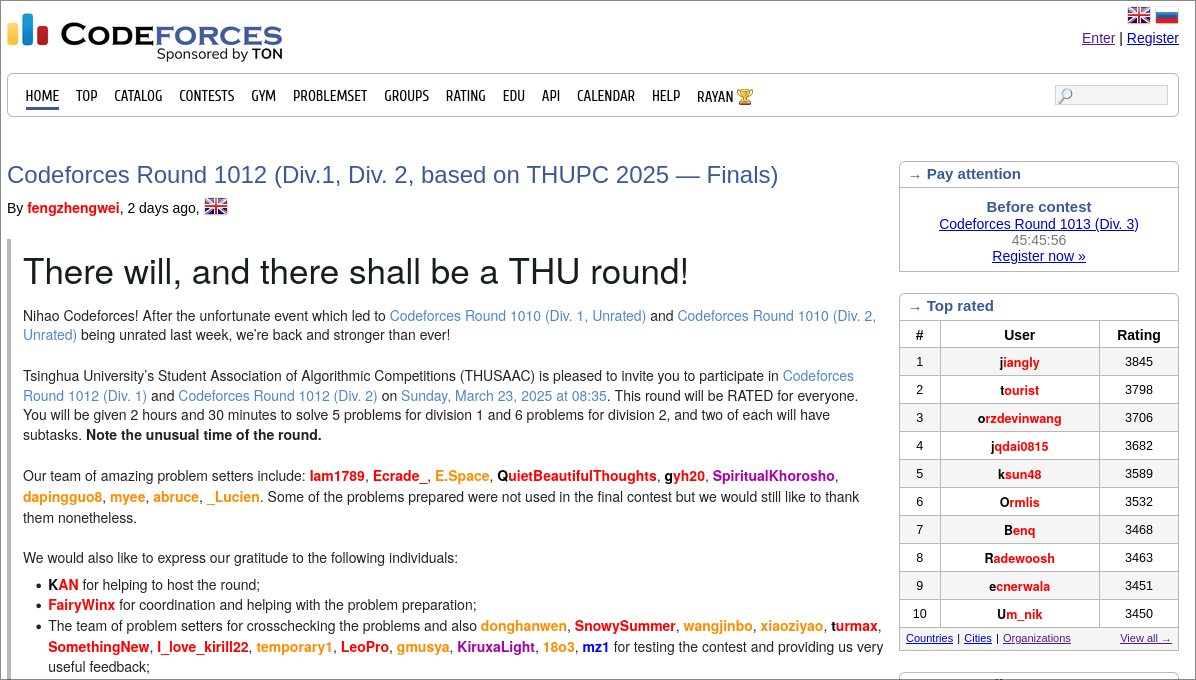
\includegraphics[]{codeforces.png}
\end{frame}

%------------------------------------------------

\begin{frame}
    \center acmp [acmp.com]

    \center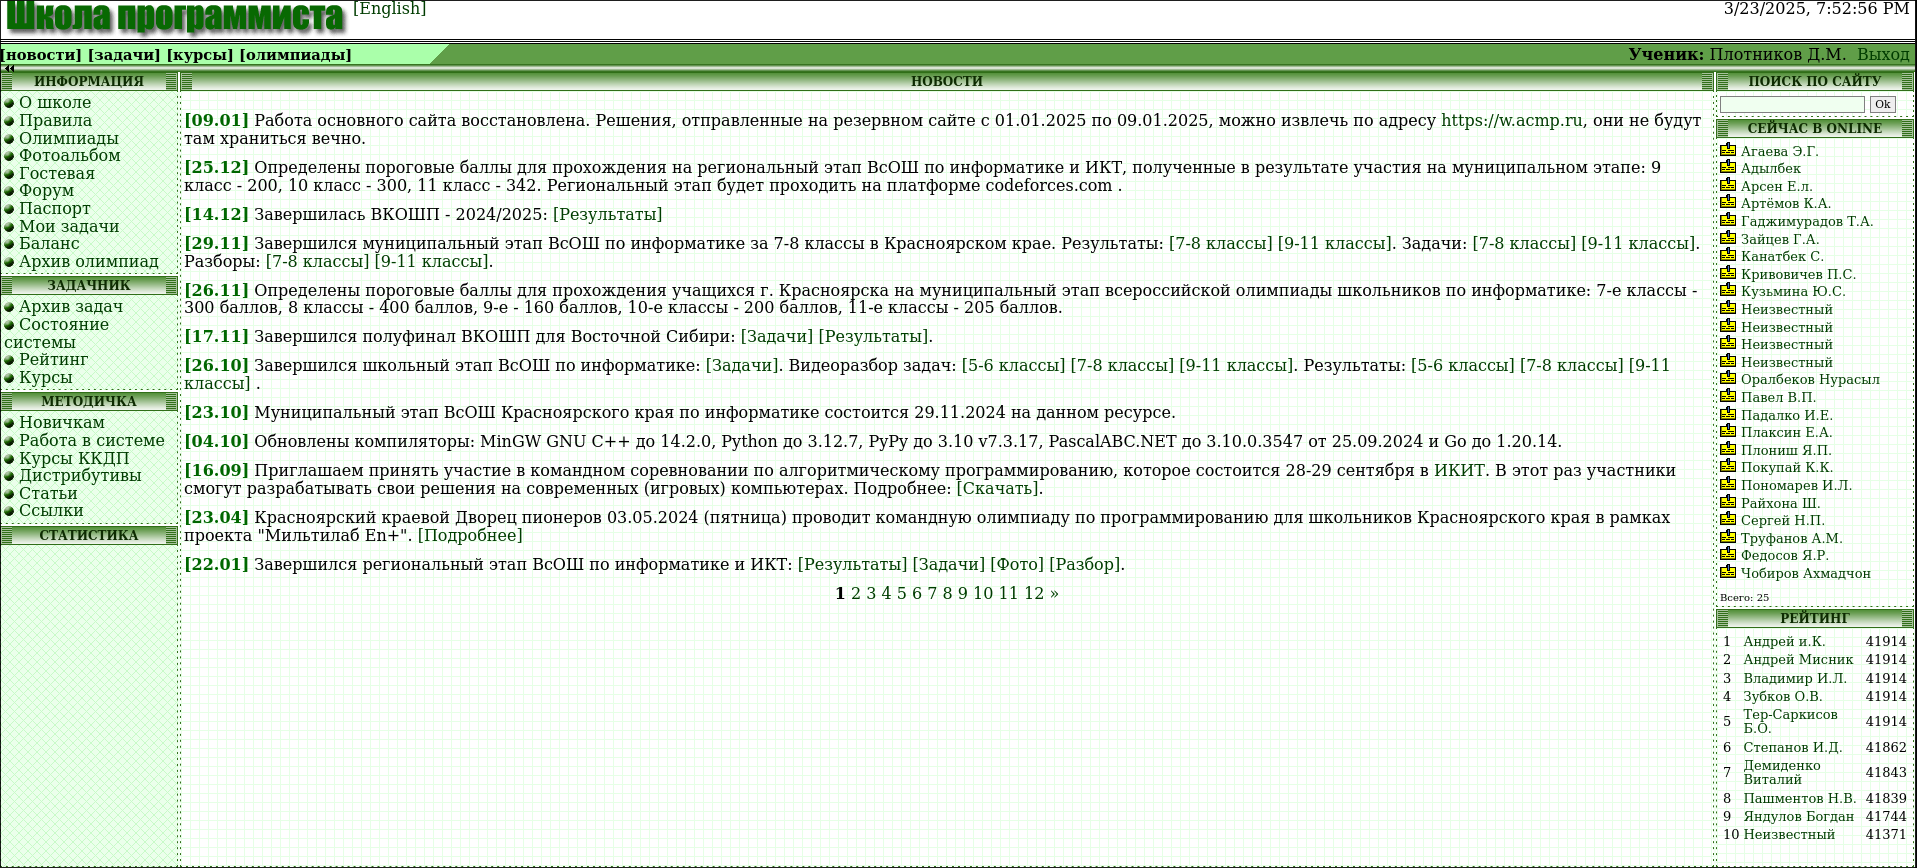
\includegraphics[scale=0.90]{acmp.png}
\end{frame}

%------------------------------------------------

\begin{frame}
    \center timus [acm.timus.ru]

    \center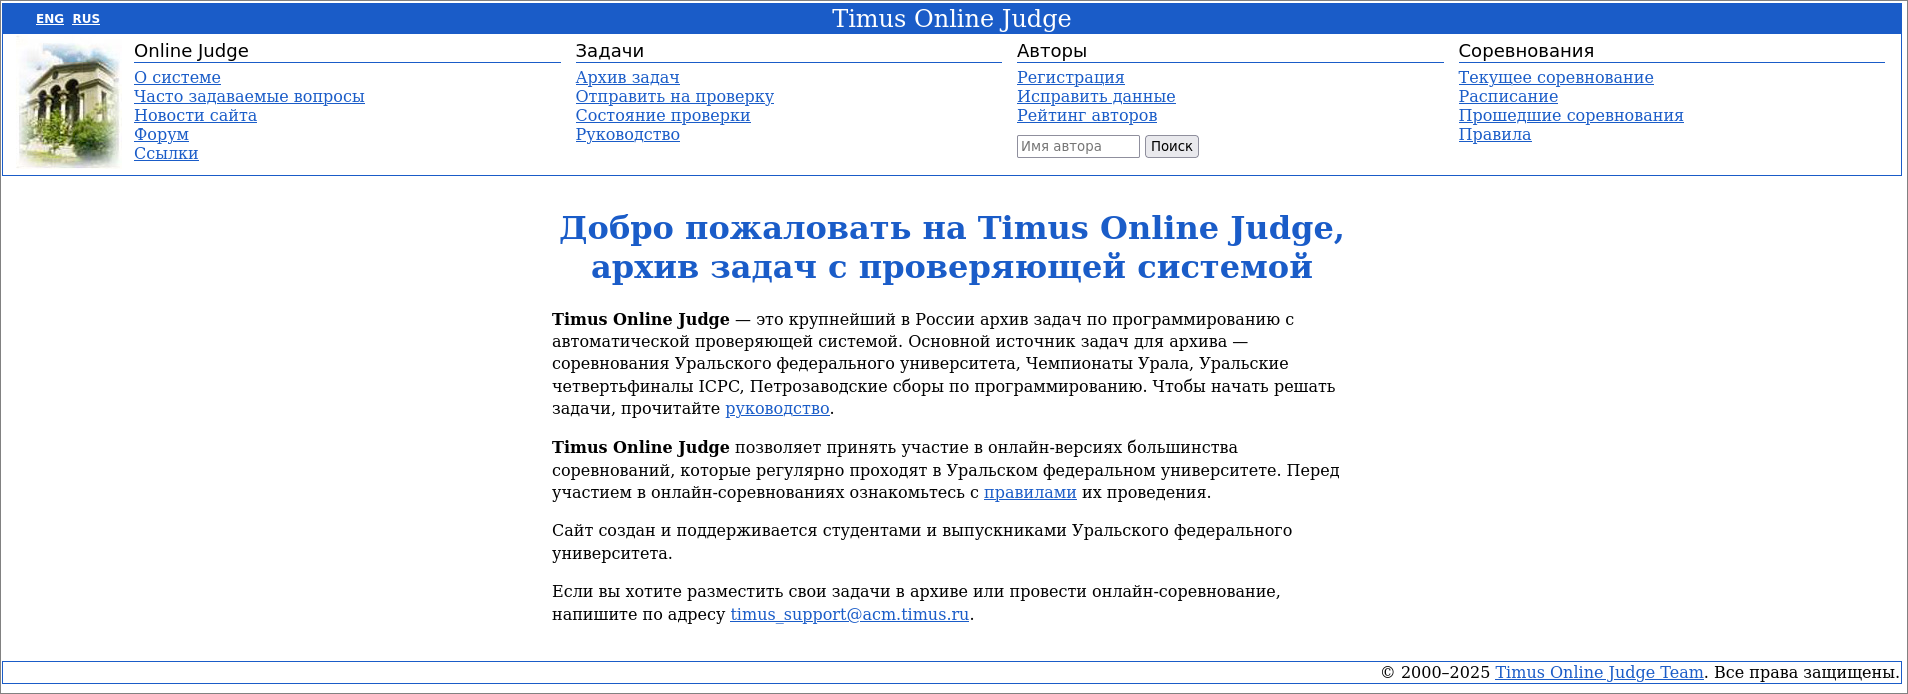
\includegraphics[scale=0.95]{timus.png}
\end{frame}

%------------------------------------------------

\begin{frame}
    \center e-maxx [e-maxx.ru/algo]

    \center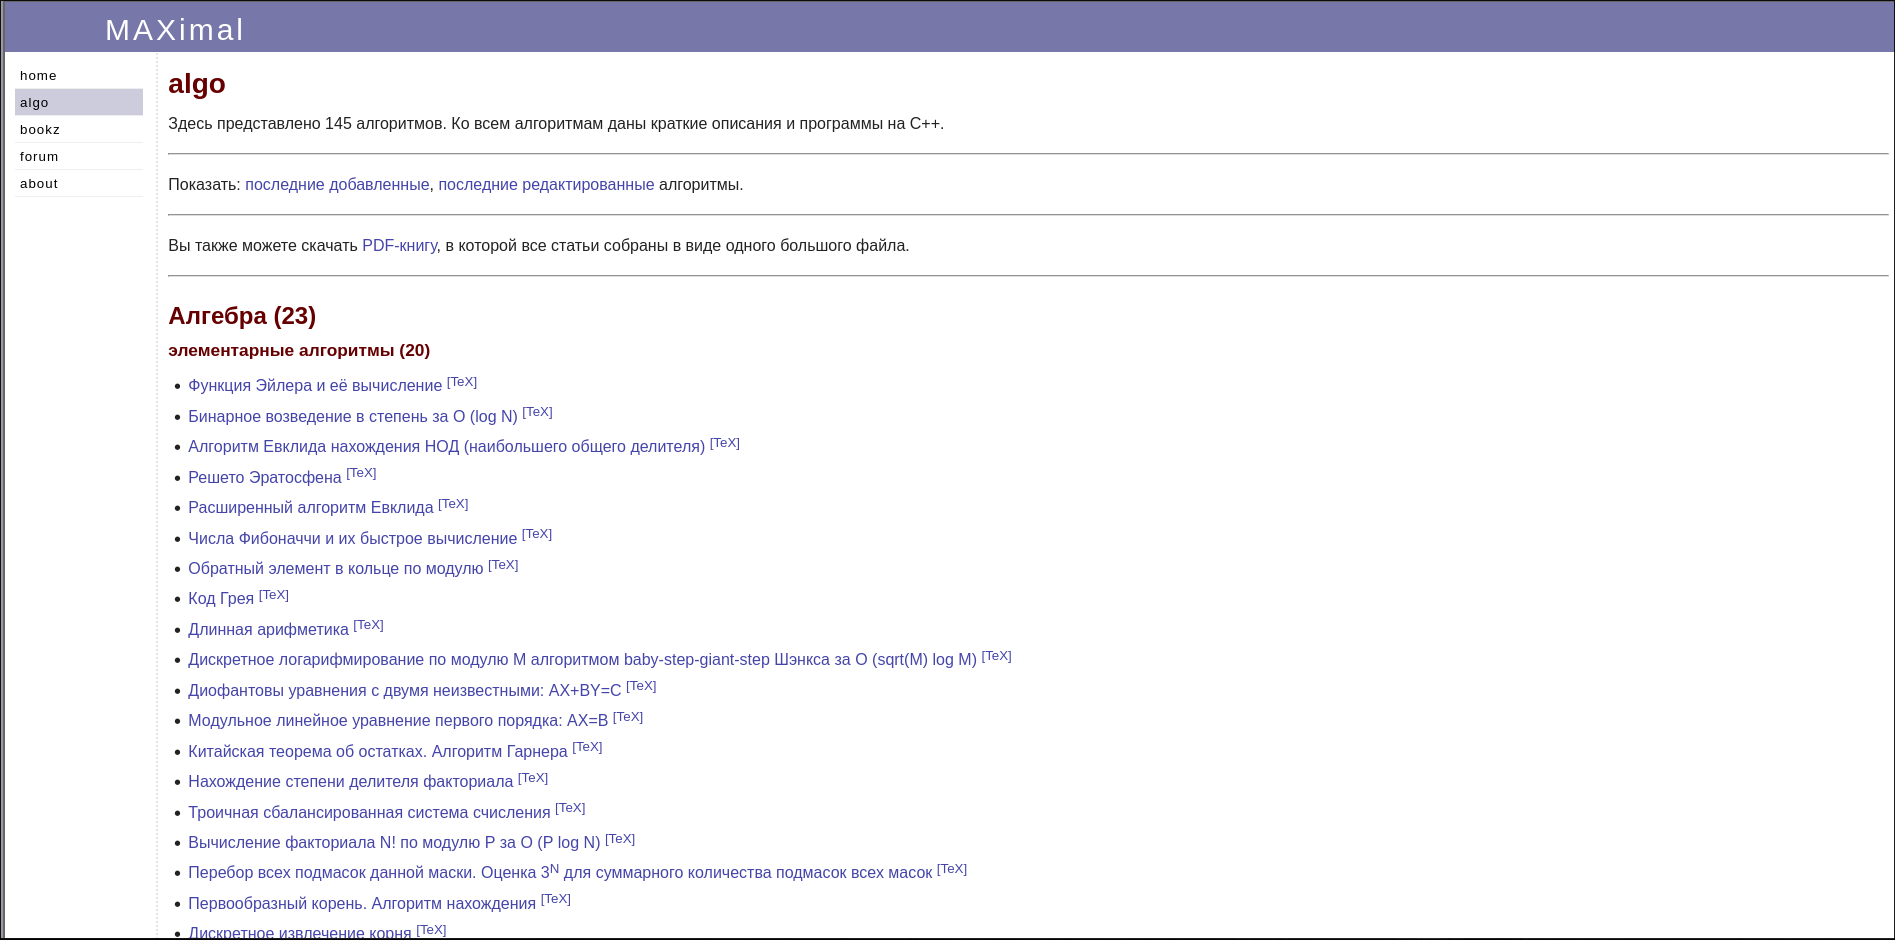
\includegraphics[scale=0.85]{e-maxx.png}
\end{frame}

%------------------------------------------------

\begin{frame}
    \center algorithmica [ru.algorithmica.org]

    \center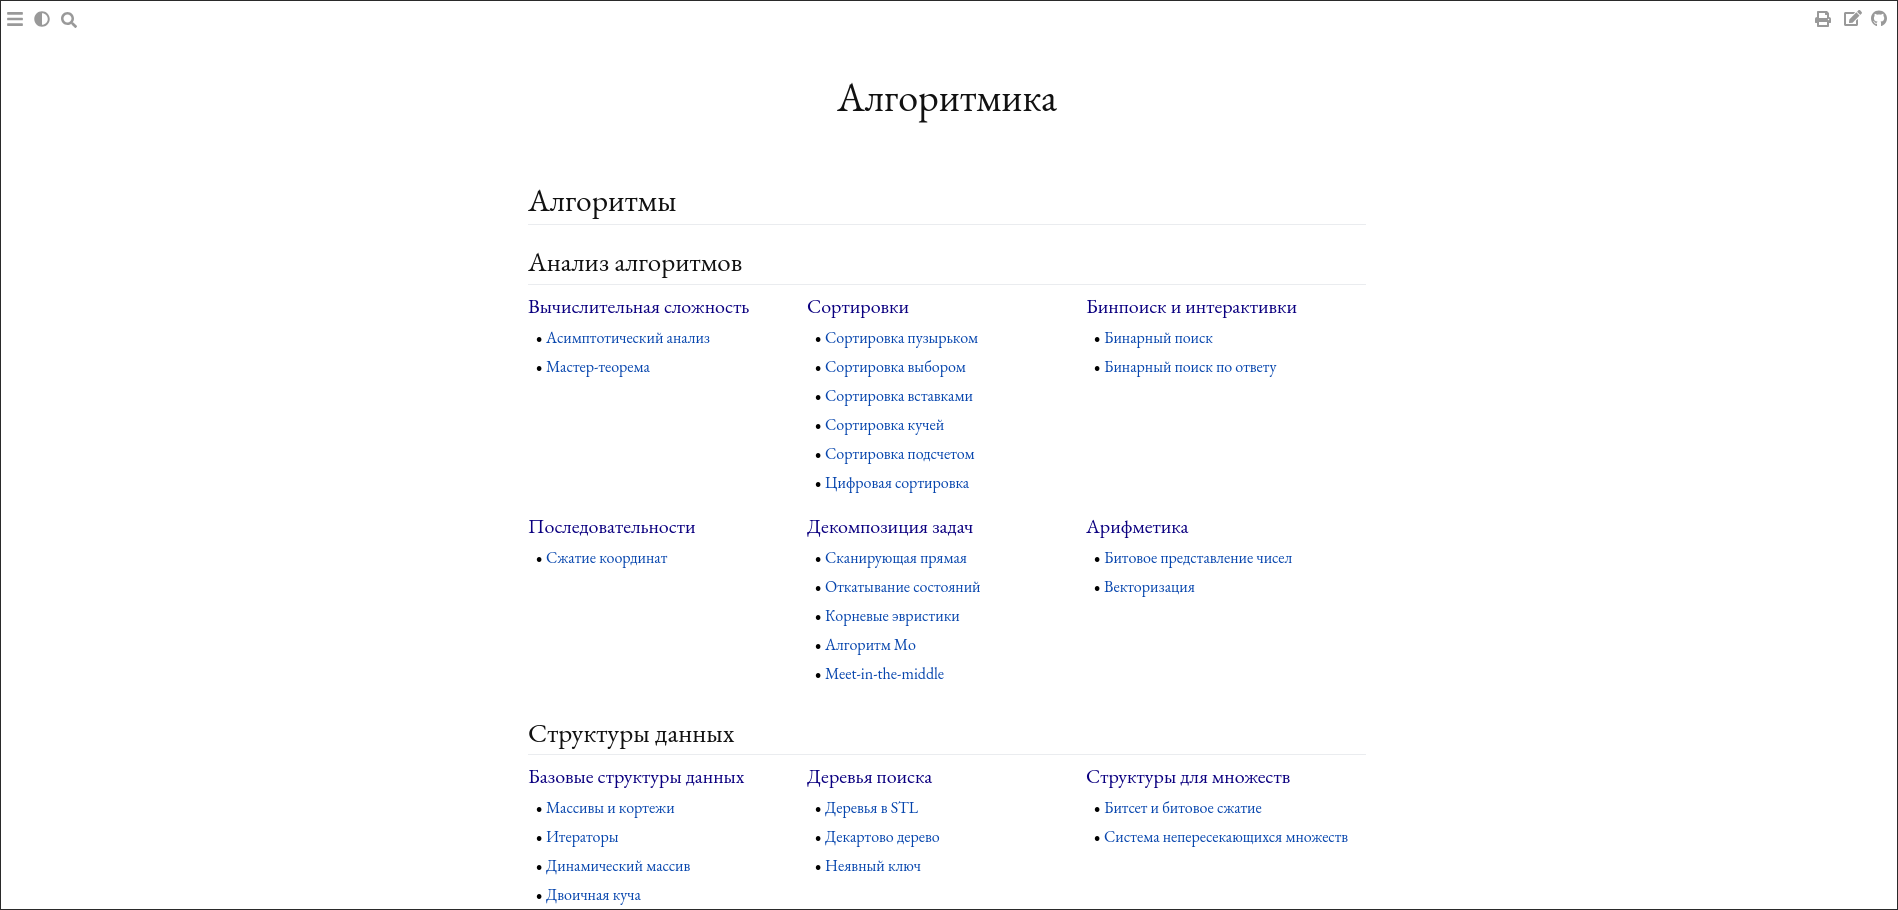
\includegraphics[scale=0.85]{algorithmica.png}
\end{frame}

%------------------------------------------------

\begin{frame}
    \center usaco [usaco.org]

    \center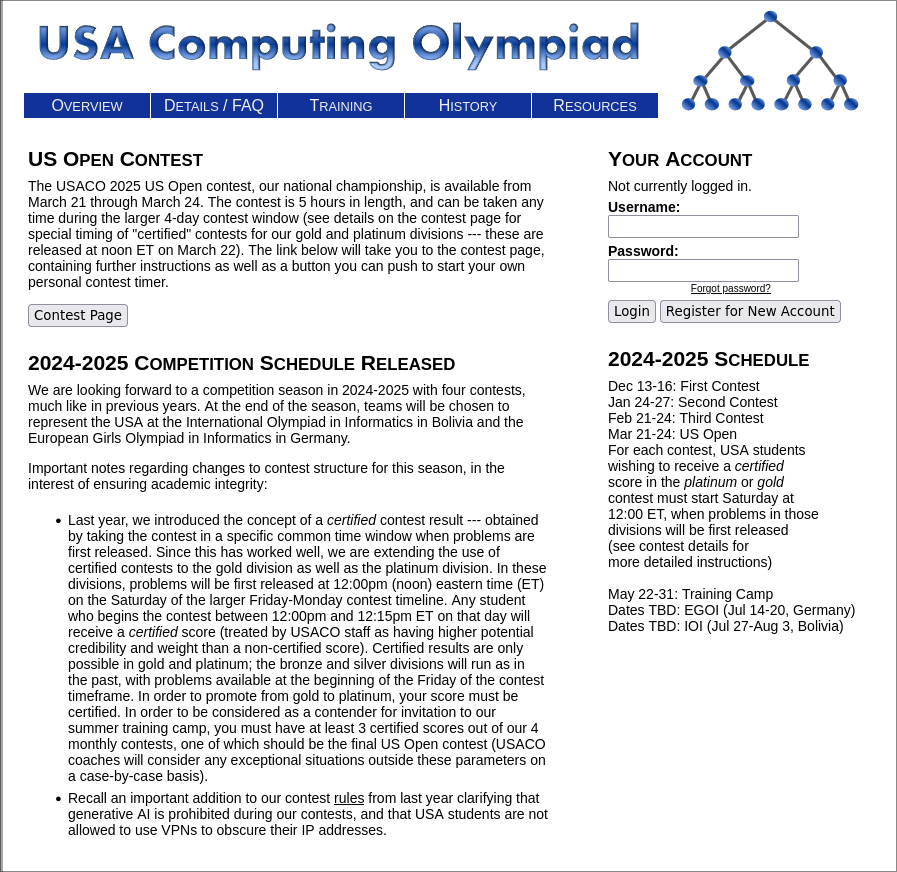
\includegraphics[scale=0.90]{usaco.png}
\end{frame}

%------------------------------------------------

\section{Асимптотика}

%------------------------------------------------

\begin{frame}
    \center \Huge Асимптотика
\end{frame}

%------------------------------------------------

\begin{frame}
    \frametitle{Логарифм}

    \big 
    $x=\log_a{b}$ это такое число x, что x^a=b

    $4=\log_4{16}$

\end{frame}

%------------------------------------------------

\begin{frame}
    \frametitle{Определение}
    \quad $g(x) = O(f(x)) => \exists C = const : \exists x_1:  \forall x\geq x_1 \Rightarrow Cg(x) \geq f(x)$ 

    \quad Функция $g(x)$ является асимптотической оценкой функции $f(x)$ тогда, когда существует константа $С$, при которой найдётся такой $x_1$, что для любого $x$, не меньшего $x_1$, выполняется неравенство $Cg(x) \geq f(x)$

\end{frame}

%------------------------------------------------

\begin{frame}
    \frametitle{Определение}

    \begin{tikzpicture}
        \begin{axis}[
            xmin=0, xmax=100,
            ymin=0, ymax=20,
            xtick={0,100},
            ytick={0,120},
            legend pos=north east,
            ]

            \addplot[
                color=blue,
                mark=none,
                samples=200,
                domain=0:100,
                unbounded coords=jump
                ]
                {sqrt(x)};

            \addplot[
                color=red,
                mark=none,
                samples=200,
                domain=0:100,
                unbounded coords=jump
                ]
                {log10(x)};

            \addplot[
                color=cyan,
                mark=none,
                samples=200,
                domain=0:100,
                unbounded coords=jump
                ]
                {x};

            \legend{$\sqrt(x)$, 
                    $\log_{10}(x)$,
                    $x$}
        \end{axis}
    \end{tikzpicture}
    \begin{tikzpicture}
        \begin{axis}[
            xmin=0, xmax=1000,
            ymin=-50, ymax=50,
            xtick={1000},
            ytick={0},
            legend pos=south west,
            fr
            ]

            \addplot[
                color=blue,
                mark=none,
                samples=200,
                domain=0:1000,
                unbounded coords=jump
                ]
                {25*sin(x)};

            \addplot[
                color=red,
                mark=none,
                samples=200,
                domain=0:1000,
                unbounded coords=jump
                ]
                {sqrt(x)};

            \addplot[
                color=black,
                mark=none,
                samples=200,
                domain=0:1000,
                unbounded coords=jump
                ]
                {0};

            \legend{$\sin(x)$, 
                    $\sqrt(x)$}
        \end{axis}
    \end{tikzpicture}

\end{frame}

%------------------------------------------------

\begin{frame}
    \frametitle{Частые асимптотики}

    \begin{center}
        \begin{tabular}{|c|c|} 
            \hline
            Асимптотика & Возможный размер данных \\
            \hline
            $a^n$ & примерно никогда \\  
            \hline
            $n!$ & 10 \\  
            \hline
            $n^3$ & 500 \\  
            \hline
            $n^2$ & 10000 \\  
            \hline
            $nlog(n)$ & 10^6 \\  
            \hline
            $n$ & 10^8 \\  
            \hline
            $\sqrt{n}$ & не хватит памяти \\  
            \hline
            $\log{n}$ & не хватит памяти \\  
            \hline
            $1$ & ваще жесть \\  
            \hline
        \end{tabular}
    \end{center}
\end{frame}

%------------------------------------------------

\begin{frame}
    \frametitle{Как считать?}

    \begin{enumerate}
        \item Заведём функцию сложности алгоритма
        \item Посчитаем примерное количество операций
        \item Держим в уме накладные расходы
        \item Придумываем худший случай
    \end{enumerate}
\end{frame}

%------------------------------------------------

\begin{frame}
    \frametitle{Свойства}

    \quad $g(x) = O(f(x)) => \exists C = const : \exists x_1:  \forall x\geq x_1 \Rightarrow Cg(x) \geq f(x)$ 

    \begin{enumerate}
        \item $a=const \Rightarrow O(af(x))=OO(f(x))$
        \item $O(n^2+n+8)=O(n^2)$\\
    \end{enumerate}

     \quad Важно помнить что на самом деле и константы и малые функции всё ещё влияют на временную сложность и могут привести к неверное оценке алгоритма 
\end{frame}

%------------------------------------------------

\begin{frame}
    \frametitle{Почему нет основания логарифма?}
    \quad $O(\log_a{n})=O(\dfrac{\log_b{n}}{\log_b{a}})=\dfrac{1}{\log_b{a}}\log_b{n}\\ \dfrac{1}{\log_b{a}}=const \Rightarrow O(\dfrac{1}{\log_b{a}}\log_b{n})=O(\log_b(n))\Rightarrow O(\log_a{n}) = O(\log_b(n))$

\\
    \quadОпять же, стоит понимать что от основания на самом деле влияет скорость выполнения и для точной оценки его следует писать
\end{frame}

%------------------------------------------------

\begin{frame}[fragile]
    \frametitle{Упражнения}
    
    Сортировка пузырьком
    \begin{cpp}
        for (int i = 0; i < arr.size(); i++) {
            for (int j = 0; j < arr.size()-1; j++) {
                if (arr[j] > arr[j + 1]) {
                    int tmp = arr[j];
                    arr[j] = arr[j + 1];
                    arr[j + 1] = b;
                }
            }
        }
    \end{cpp}
    
\end{frame}

%------------------------------------------------

\begin{frame}[fragile]
    \frametitle{Упражнения}
    
    Сортировка пузырьком
    \begin{cpp}
        for (int i = 0; i < arr.size(); i++) {
            for (int j = 0; j < arr.size()-1; j++) {
                if (arr[j] > arr[j + 1]) {
                    int tmp = arr[j];
                    arr[j] = arr[j + 1];
                    arr[j + 1] = b;
                }
            }
        }
    \end{cpp}

    Ответ: $O(n^2)$

\end{frame}

%------------------------------------------------

\begin{frame}[fragile]
    \frametitle{Упражнения}
    
    \begin{cpp}
        int recursion(n){
            if(n < 1){
                return 1;
            }

            int ans = 0;
            for(int i = 0; i < n){
                ans += recursion(n);
            }

            return ans;
        }
    \end{cpp}
    
\end{frame}

%------------------------------------------------

\begin{frame}[fragile]
    \frametitle{Упражнения}
    
    \begin{cpp}
        int recursion(int n){
            if(n < 1){
                return 1;
            }

            int ans = 0;
            for(int i = 0; i < n){
                ans += recursion(n);
            }

            return ans;
        }
    \end{cpp}
    
    Ответ: $O(n^n)$
\end{frame}

%------------------------------------------------

\begin{frame}[fragile]
    \frametitle{Упражнения}
    
    Дерево Фенвика
    \begin{cpp}
        int sum (int r){
            int result = 0;
            for (int i = r; i >= 0; r = (i & (i+1)) - 1){
                result += t[r];
            }
            return result;
        }
    \end{cpp}
    
\end{frame}

%------------------------------------------------

\begin{frame}[fragile]
    \frametitle{Упражнения}
    
    Дерево Фенвика
    \begin{cpp}
        int sum (int r){
            int result = 0;
            for (int i = r; i >= 0; r = (i & (i+1)) - 1){
                result += t[r];
            }
            return result;
        }
    \end{cpp}
    
    Ответ: $O(log{n})$
\end{frame}

%------------------------------------------------

\begin{frame}[fragile]
    \frametitle{Упражнения}
    
    Дерево Отрезков
    \begin{cpp}
        int sum (int v, int tl, int tr, int l, int r) {
            if (l > r){
                return 0;
            }
            if (l == tl && r == tr){
                return t[v];
            }
            int tm = (tl + tr) / 2;
            return sum (v*2, tl, tm, l, min(r,tm))
            + sum (v*2+1, tm+1, tr, max(l,tm+1), r);
        }
    \end{cpp}
    
\end{frame}

%------------------------------------------------

\begin{frame}[fragile]
    \frametitle{Упражнения}

    Дерево Отрезков
    \begin{cpp}
        int sum (int v, int tl, int tr, int l, int r) {
            if (l > r){
                return 0;
            }
            if (l == tl && r == tr){
                return t[v];
            }
            int tm = (tl + tr) / 2;
            return sum (v*2, tl, tm, l, min(r,tm))
            + sum (v*2+1, tm+1, tr, max(l,tm+1), r);
        }
    \end{cpp}
    
    Ответ: $O(log{n})$
\end{frame}

%------------------------------------------------

\begin{frame}
    \center\huge{Ссылка на тест в телеграме}
    \center
\includegraphics[scale=0.15]{QRtest.png}
\end{frame}

%------------------------------------------------

\section{Основы}

%------------------------------------------------

\begin{frame}
    \center \Huge Основы
\end{frame}

%------------------------------------------------

\begin{frame}
    \frametitle{Целые числа}

    существуют

    полезные
\end{frame}

%------------------------------------------------

\begin{frame}
    \frametitle{Целые числа. Представление числа}
    Числа представляются в двоичной системе счисления

    \begin{itemize}
        \item 0 = 00000000
        \item 8 = 00001000
        \item 53 = 00110101
        \item 255 = 01111111
    \end{itemize}
\end{frame}

%------------------------------------------------

\begin{frame}
    \frametitle{Целые числа. Побитовые операции}

    \begin{tabular}{cc}
        \begin{minipage}{.5\linewidth}
            \begin{table}[h!]
                Побитовое не \sim \\
                \begin{tabular}{|c|c|}
                    \hline
                    a & \sim a \\ [0.5ex]
                    \hline\hline
                    0    & 1    \\
                    1    & 0    \\
                    \hline
                \end{tabular}
            \end{table}
        \end{minipage}

        \begin{minipage}{.4\linewidth}
            \begin{table}[h!]
                Побитовое и \& \\
                \begin{tabular}{|c|c|c|}
                    \hline
                    a & b & a\&b \\[0.5ex]
                    \hline\hline
                    0 & 0 & 0  \\
                    0 & 1 & 0  \\
                    1 & 0 & 0  \\
                    1 & 1 & 1  \\
                    \hline
                \end{tabular}
            \end{table}
        \end{minipage}
    \end{tabular}
\end{frame}

%------------------------------------------------

\begin{frame}
    \frametitle{Целые числа. Побитовые оперцаии}

    \begin{tabular}{cc}
        \begin{minipage}{.5\linewidth}
            \begin{table}[h!]
                Побитовое или | \\
                \begin{tabular}{|c|c|c|}
                    \hline
                    a & b & a\&b \\[0.5ex]
                    \hline\hline
                    0 & 0 & 0  \\
                    0 & 1 & 1  \\
                    1 & 0 & 1  \\
                    1 & 1 & 1  \\
                    \hline
                \end{tabular}
            \end{table}
        \end{minipage}

        \begin{minipage}{.4\linewidth}
            \begin{table}[h!]
                Побитовый xor \^ \\
                \begin{tabular}{|c|c|c|}
                    \hline
                    a & b & a\&b \\[0.5ex]
                    \hline\hline
                    0 & 0 & 0  \\
                    0 & 1 & 1  \\
                    1 & 0 & 1  \\
                    1 & 1 & 0  \\
                    \hline
                \end{tabular}
            \end{table}
        \end{minipage}
    \end{tabular}
\end{frame}

%------------------------------------------------

\begin{frame}
    \frametitle{Целые числа. Побитовые оперции}

    \begin{center}
        Побитовый сдвиг вправо >> и побитовый сдвиг влево <<: \\
        00010101 << 1 = 00101010 \\
        21 << 1 = 42 = 21 \times $2^1$ \\
        0000011010100111 >> 1 = 0000001101010011 \\
        1703 >> 1 = 851 = 1703 / $2^1$ \\
    \end{center}

\end{frame}

%------------------------------------------------
\begin{frame}
    \frametitle{Целочисленные типы данных в языке с++}

    \begin{center}
        \small
        \begin{tabular}{|c|c|c|}
            \hline
            Тип & Размер & Значения \\
            \hline
            short int & 16 & -32,768 --- 32,767\\
            \hline
            unsigned short int & 16 & 0 --- 65,535\\
            \hline
            int & 32 & -2,147,483,648 --- 2,147,483,647\\
            \hline
            unsigned int & 32 & 0 -- 4,294,967,295\\
            \hline
            long int & 32 & -2,147,483,648 --- 2,147,483,647\\
            \hline
            unsigned long int & 32 & 0 -- 4,294,967,295\\
            \hline
            long long int & 64 & -9,223,372,036,854,775,808 --- 9,223,372,036,854,775,807\\
            \hline
            unsigned long long int & 64 & 0 --- 18,446,744,073,709,551,615\\
            \hline
        \end{tabular}
    \end{center}

    \quad Модификаторы: short, long, signed, unsigned\\
    \quad При подключении заколовочного файла <cstdint> можно писать int[8/16/32/64]\_t и uint[8/16/32/64]\_t
\end{frame}

%------------------------------------------------

\begin{frame}
    \frametitle{Отрицательные целые числа}
    \quad Очевидная запись: от всех чисел отнимать константу. Эта константа будет минимальных числом.

    \quad Пример: пусть константа 52, а в памяти записано в двоичном виде число 42. Значит фактически число в этой переменной 42-52=-10   

    \quad Решение рабочее, но медленное и неудобное.

    \quad Как же хранится число на самом деле? 

    \quad Первый(самый старший) бит числа отвечает за знак. Тогда чтобы из положительного получить отрицателное нужно сделать операцию $-a = \sim a - 1$ но чем же это лучше?
\end{frame}

%------------------------------------------------

\begin{frame}
    \frametitle{Переполнения целых чисел}

    \quad Что будет если в восьмибитном знаковом числе сложить 89 и 100? Максимальное число это 127, что меньше этой суммы. Ответом будет -67.

    \quad Вернёмся к представлению числа чтобы понять почему так происходит.

    \quad $87 = 01010111$\\
    \quad $100 = 01100100$\\
    \quad $100 + 87 = 187 = 10111011$, что при первом бите ответственном за знак является $10111011 = -(01000100 - 00000001) = -67$. Не выглядит удобным. В чём же польза?

\end{frame}

%------------------------------------------------

\begin{frame}
    \frametitle{Переполнения целых чисел}

    \quad Рассмотрим сумму чисел разных знаков

    \quad $-87 = 10101001$\\
    \quad $100 = 01100100$\\
    \quad $10101001 + 01100100 = 00001101 = 13$. Сумма сработала без каких либо дополнительных операций. Подобным свойством обладают также разность, умножение и деление. Фактически реализация разности и деления вовсе необязательна. На этом факте строиться Дерево Фенвика из примера асимптотического анализа алгоритма.

\end{frame}

%------------------------------------------------

\begin{frame}[fragile]
    \frametitle{Ввод и вывод}

    \begin{cpp}
        #include <iostream>
        using namespace std;
        int main(){
            std::ios_base::sync_with_stdio(0);
            cin.tie(0);
            cout.tie(0);

            string s;
            cin >> s;
            cout << "Hello, mister " << s << "!";

            cout.flush();
            cout << "\n" << std::endl;
            
            return 0;
        }
    \end{cpp}
\end{frame}

%------------------------------------------------

\begin{frame}[fragile]
    \frametitle{Ввод и вывод}
    Ускорение ввода и вывода
    \begin{cpp}
            std::ios_base::sync_with_stdio(0);
            cin.tie(0);
            cout.tie(0);
    \end{cpp}

    Очистка буфера
    \begin{cpp}
            cout.flush();
    \end{cpp}

    НЕ ОДНО И ТО ЖЕ!!!
    \begin{cpp}
            cout << "\n";
            cout << endl;
    \end{cpp}
    
\end{frame}

%------------------------------------------------

\begin{frame}[fragile]
    \frametitle{Строки}
    
    \quad Под капотом строки на самом деле это не более чем массив символов с одной особенностью. В конце находится терминальный символ с значением 0. Такую записать можно представить так:
    \begin{cpp}
        char a[4] = {'1', '2', '3', 0};
        char b[4] = {'1', '2', '3', '\0'};
    \end{cpp}
\end{frame}

%------------------------------------------------

\section{pref\_sum}

%------------------------------------------------

\begin{frame}
    \center \Huge Массив префиксных сумм
\end{frame}

%------------------------------------------------

\begin{frame}[fragile]
    \center\huge{Задача}

    \normalsize
    \quad Есть массив. Требуется найти сумму всех элементов, индексы которых находятся в промежутке [l,r].

    \centering
    Входные данные:
    \begin{cpp}
10 
1 2 3 4 5 6 7 8 9 10 
4 
1 4
3 6
6 7
1 10
    \end{cpp}
\end{frame}

%------------------------------------------------

\begin{frame}[fragile]
    \begin{cpp}
int n; cin >> n;
vector<int> a(n),b(n+1);
for(int i = 0; i < n; ++i){
    cin >> a[i];
}
b[0] = 0;
for(int i = 1; i <= n; ++i){
    b[i] = b[i-1] + a[i-1];
}
int t; cin >> t;
for(int i = 0; i < n; ++i){
    int l, r; cin >> l >> r;
    cout << b[r] - b[l-1] << '\n';
}
    \end{cpp}
\end{frame}

%------------------------------------------------


%------------------

\end{document}

